%% muKV, 6-page version (HotMobile: 6 pages plus references) (2026-09-07). Built from PAPER_HOTMOBILE_2027.tex (source of truth for
%% every number). Structure: intro, background, design, control, implementation, evaluation,
%% related work, conclusion. No em dashes; captions under 35 words; table captions above.
\documentclass[sigconf, anonymous=false, screen=true]{acmart}
\settopmatter{printacmref=false}
\renewcommand\footnotetextcopyrightpermission[1]{}
\pagestyle{plain}
\acmConference[HotMobile '27]{International Workshop on Mobile Computing Systems and Applications}{2027}{}
\usepackage{booktabs}
\usepackage{multirow}
\newcommand{\yes}{$\bullet$}
\newcommand{\no}{$\cdot$}
\usepackage{xcolor}
\usepackage{hyperref}
\usepackage{microtype}
\usepackage{graphicx}
\graphicspath{{figures/}}
\usepackage{enumitem}
\newcommand{\slb}{/\allowbreak}
\newcommand{\ub}{\_\allowbreak}
\setlength{\emergencystretch}{2em}
\definecolor{kvgreen}{RGB}{40, 174, 96}
\definecolor{kvred}{RGB}{192, 57, 43}
\definecolor{kvgray}{RGB}{85, 85, 85}
\newcommand{\good}[1]{\textcolor{kvgreen}{\textbf{#1}}}
\newcommand{\bad}[1]{\textcolor{kvred}{\textbf{#1}}}
\newcommand{\muKV}{$\mu$KV}
\newcommand{\C}{\,\textdegree C}

\begin{document}

\title[\muKV: Energy- and Thermal-Aware KV Eviction on a Phone]{\muKV: Energy- and Thermal-Aware KV-Cache Eviction for LLM Inference on a Phone}

\author{Md Romyull Islam}
\affiliation{%
  \institution{Kennesaw State University}
  \city{Marietta}
  \state{Georgia}
  \country{USA}
}
\email{romyullislam2012@gmail.com}

\begin{abstract}
On a phone the KV cache, not compute, limits sustained LLM decode. The policies that bound it were built for server GPUs. Three properties of a real on-device engine break them. One cell array serves every head and layer, so a cell is freed only when every head and every layer drops it. SnapKV reports an 8.2 times smaller cache; on this engine it retains 68\% of the cells at a matched budget and 94\% at its own. Reading attention scores forces the FlashAttention-off path, so score-reading evictors decode at 0.12 to 0.30 times the full cache on the phone GPU. Compaction through the state API needs a second full context, and the OS kills Phi-3-mini at 16K. \muKV\ scores tokens inside the FlashAttention prefill graph through a small side node, selects one keep set for all heads and layers, and compacts in place. A reduce-only clock watchdog with CPU and GPU ladders keeps the vendor throttle unreachable. A per-request scheduler picks the GPU clock plan, the cache budget and the answer cap from the battery state, and two loops correct it. On a OnePlus 15, \muKV\ decodes 4.8 times faster than the full cache on the CPU and 1.23 times on the Adreno GPU, at 7\% of the cells and 62\% less energy. It ties the full cache on 392 retrieval cells and stays within 0.1 to 3.7 F1 on LongBench at 13\% of the cache. Through a real discharge from 91 to 11\%, its two lower tiers cut energy per request by 15\% and 43\%.
\end{abstract}

\keywords{Mobile LLM inference, KV cache eviction, FlashAttention, thermal management, energy-aware scheduling, on-device AI}

\maketitle
\makeatletter\fancyhead[RO]{\@headfootfont HotMobile '27}\fancyhead[LE]{\@headfootfont HotMobile '27}\makeatother

\section{Introduction}
\label{sec:intro}

Small instruction-tuned models now run interactively on flagship phones. For a sustained generation the wall is the KV cache, not the matrix multiply. Every decode step reads the whole cache once per layer. Past a thousand tokens the step is bound by DRAM bandwidth. The DRAM heats, the vendor thermal engine cuts the clock, and the battery drains. Cache size sets traffic, traffic sets power, power sets temperature, temperature sets the throttle, and the throttle sets throughput. A mobile cache policy must therefore be judged on quality, throughput, heat and energy together, on real hardware.

The policies that bound the cache were built for server GPUs and judged by perplexity alone: H2O~\cite{zhang2023h2o}, TOVA~\cite{oren2024tova}, SnapKV~\cite{li2024snapkv}, StreamingLLM~\cite{xiao2024streamingllm} and Ada-KV~\cite{feng2025adakv}. We ran each in its published configuration on a OnePlus 15 inside \texttt{llama.cpp}. Three properties of the engine broke them.

\begin{itemize}[leftmargin=*, itemsep=1pt]
\item \textbf{Budgets do not materialize.} The engine keeps one cell array shared by every head and layer. A cell is freed only when every head and every layer drops it. SnapKV selects per head and reports an 8.2 times smaller cache at 16K inputs~\cite{li2024snapkv}. At a matched budget of 1024 per head on this engine it keeps 68\% of the cells on Llama-3.2-1B and 85\% on Phi-3-mini. At its own budget of 2048 per head it keeps 94\%. H2O reports a 5 to 10 times smaller cache at a 20\% budget~\cite{zhang2023h2o}; at that budget here it keeps 92 to 99.8\%.
\item \textbf{Scores cost the fast path.} A policy that reads post-softmax attention cannot use the fused FlashAttention kernel. Every score-reading evictor decodes at 0.12 to 0.30 times the full cache on the phone GPU. Evicting makes it slower.
\item \textbf{Compaction doubles memory.} The state API restores survivors into a second context. Phi-3-mini at 16K needs two 6.4\,GB caches plus 2.4\,GB of weights, and the OS kills it. The same call fails on a 24\,GB desktop GPU.
\end{itemize}

\muKV\ is an evictor designed around these facts, with the two controllers a phone needs beside it (Figure~\ref{fig:architecture}). It computes selection scores inside the FlashAttention prefill graph through a small side node. It selects one keep set of $K$ cells for all heads and layers, so eviction frees cells. It compacts in place: survivors slide into a dense prefix inside the tensors prefill already allocated. A reduce-only watchdog steps the CPU and GPU clocks down along temperature ladders anchored at the measured vendor triggers. A per-request scheduler picks the GPU clock plan, the cache budget and the answer cap from the battery state. It predicts the request's cost from a measured table, and two loops correct its lever when time or energy misses.

We evaluate on a OnePlus 15 (Snapdragon 8 Elite Gen 5, Adreno 840) with four models and nine policies, on quality, throughput, heat and energy at once. This paper makes five contributions.

\begin{enumerate}[label=(\roman*), leftmargin=*, itemsep=1pt]
\item The realizability gap: nominal per-head budgets do not compact on a sequence-level engine, measured for five policies on four models (\S\ref{sec:eval-cpu}, \S\ref{sec:eval-gpu}).
\item In-graph scoring, one keep set and in-place compaction, which keep an attention-driven evictor on the FlashAttention path and make an infeasible configuration run (\S\ref{sec:design}).
\item A thermal watchdog with CPU and GPU ladders anchored at the measured vendor trigger, and the negative result that cache size does not cap peak temperature (\S\ref{sec:control}, \S\ref{sec:eval-thermal}).
\item An energy-aware scheduler with one lever and two loops, measured through a real battery discharge and under provoked disturbances (\S\ref{sec:eval-energy}).
\item A multi-axis on-device evaluation with every baseline in its own published configuration (\S\ref{sec:eval}).
\end{enumerate}

\section{Background}
\label{sec:bg}

H2O~\cite{zhang2023h2o} keeps heavy hitters by accumulated attention plus recent tokens and reports a 5 to 10 times smaller cache at a 20\% budget. TOVA~\cite{oren2024tova} drops the least-attended position per layer every step and reports full quality at one eighth of the cache. SnapKV~\cite{li2024snapkv} freezes a per-head top-$K$ at the end of prefill and reports an 8.2 times smaller cache at 16K inputs. StreamingLLM~\cite{xiao2024streamingllm} keeps 4 sinks and a sliding window with no scores and states that it adds no long-term memory. Ada-KV~\cite{feng2025adakv} allocates one layer budget across heads and needs FlashAttention-2's variable-length kernel~\cite{dao2023flashattention2} plus a custom CUDA kernel, both absent on the mobile stack. FlashAttention~\cite{dao2022flashattention} fuses softmax into the kernel and never writes the attention tensor, so a policy that reads scores is locked to the slow path. \texttt{llama.cpp}~\cite{llamacpp}, like every on-device engine we know of, stores the cache as one array of position-indexed cells shared across heads and layers. It removes cells by position and compacts through a state API that restores into a second context. Neither fact is visible on a server with per-head paged storage.

On the control side, zTT~\cite{kim2021ztt} and FUSE~\cite{liu2022fuse} govern frequency from temperature or phase, with no cache or battery signal. The vendor engine on our SoC deep-throttles the prime cores to 883\,MHz the moment the battery reaches 50\C\ and caps the GPU at 726\,MHz when DDR passes 64\C. No shipped phone changes an LLM's clock, context or answer length by battery state. EnerInfer~\cite{zou2026enerinfer}, the closest research system, excludes battery level by design. Kim, Imes and Hoffmann~\cite{kim2015racepace} prove that an energy-optimal schedule under a deadline uses at most two configurations. JouleGuard~\cite{hoffmann2015jouleguard} couples two loops through model error. \muKV's scheduler applies both.

\begin{figure*}[tp]
\centering
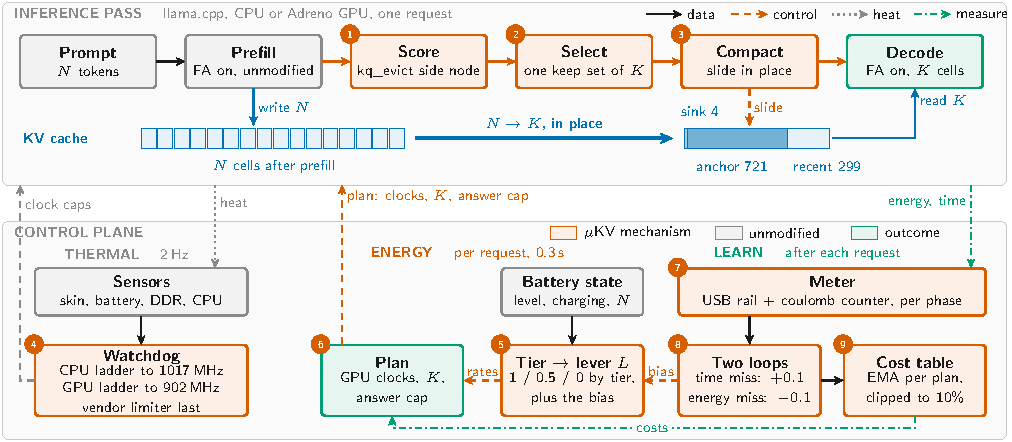
\includegraphics[width=0.96\textwidth]{fig_architecture_tikz.pdf}
\caption{\muKV\ on the phone. Top: the inference pass, with scoring, selection and compaction (1 to 3) as the only changes. Bottom: the thermal, energy and learning columns of the control plane (4 to 9).}
\label{fig:architecture}
\end{figure*}

\section{\muKV\ Design}
\label{sec:design}

\paragraph{Scoring inside the FlashAttention graph.} The fused kernel never materializes attention. \muKV\ adds a \texttt{kq\_evict} side node to the prefill graph instead of leaving the fast path. The node computes $\mathrm{softmax}(KQ^{\top})$ for the last 16 queries of the last prefill chunk and reduces it to one score per layer, head and position, $\bar A_{l,h,p}$. It is a graph output, so the mid-graph interception that corrupts this Vulkan backend cannot touch it. It costs 1.2\% of prefill on the CPU (paired, $n{=}29$) and 138 against 131\,s on the GPU. Selection is bit-identical to a FlashAttention-off capture.

\paragraph{One keep set for all heads and layers.} Selection is sequence-level. The position score is the mean of $\bar A_{l,h,p}$ over layers and heads, max-pooled over 7 positions so a run of related tokens survives together (SnapKV's clustering step). A per-prompt split $\alpha_a$, the fraction of attention mass outside the recent window (floored at 0.70, capped at 0.95), sets how many of the $K$ cells are distant anchors; the rest is the recent window. The top $n_\mathrm{anchor}$ positions by pooled score survive, plus four sink tokens~\cite{xiao2024streamingllm}. The result is one set of $K$ positions shared by every head and layer, which is what lets the cache compact. On the 9737-token prompt $\alpha_a = 0.71$, so $K{=}1024$ is 4 sinks, 721 anchors and 299 recent cells. Earlier versions also sized a per-head budget from each head's peak attention through a closed-form ramp. Its candidate pool holds 96.5 to 99.8\% of the prompt at $K{=}1024$ on every cell. Bypassing it leaves the keep set identical (721 of 721 positions) and the output identical, so it is removed. $K$ itself is sized from the request's demand, the larger of a retrieval floor and a generation floor. In a controlled test the budget that still retrieves a fact scales with the generated span, from 256 cells at 64 tokens to 4096 at 2048, not with the prompt.

\paragraph{In-place compaction and decode.} Compaction through the state API doubles peak cache memory at the instant of restore. Phi-3-mini at 16K needs $2\times6144$\,MiB plus 2.4\,GB of weights, and Android killed the process and six co-resident apps, twice. \texttt{endurkv\_compact\_seq()} instead slides survivors into a dense prefix in bounded chunks inside the tensors prefill already allocated. Peak memory does not rise, the configuration runs at 874 cells, and the two modes produce identical keep sets (perplexities agree to 0.15\% across four model families). Decode runs over the $K$-cell cache with the fused kernel. The keep set stays frozen while the recent window slides. A re-eviction fires when the live cache exceeds $1.25\times$ its budget, which bounds the decode mean near 2K cells on a 4K generation.

\paragraph{Reduce-only clock watchdog.} A daemon samples skin, battery, DDR and CPU temperature at 2\,Hz and lowers a clock cap one step at a time, never raising it. The ladders are anchored at the measured vendor triggers. Battery 47.0 to 49.5\C\ and skin 50.0 to 52.5\C\ map to CPU caps of 1497 down to 1017\,MHz, above the 883\,MHz cliff the vendor applies at 50\C. DDR 60, 62 and 63.5\C\ map to GPU caps of 1050, 967 and 902\,MHz, below the vendor's 726\,MHz trip at 64\C. The kernel applies the lower of the user cap and the vendor cap, so the ladders act earlier than the vendor and never later. On a cold phone they stay dormant.

\paragraph{Energy-aware scheduling: one lever, two loops.} Once per request, in 0.3\,s, the scheduler reads the battery level, the charging state, the prompt length, and whether the caller fixed an answer length. A tier follows (mains or above 50\%, 21 to 50\%, 20\% or below) and sets a lever $L\in\{1,0.5,0\}$ plus a learned bias. $L$ fixes every rate the scheduler trades at. The exchange rate a step must beat is 1.5, 0.8 or 0.5\,J saved per second given up. A quality floor and a time slack follow it, and so does the answer cap when the length is open: 4096, 1024 or 512 tokens. A measured cost table predicts energy and time per plan. A plan is a GPU clock cap for prefill, one for decode and the cache budget. The walk down the ladder takes a step only if the predicted saving beats the exchange rate inside the time budget. After the request, if time ran more than 5\% over the budget the plan was chosen under, the performance loop moves the bias 0.1 toward performance. If energy ran more than 5\% over its prediction, the energy loop moves it 0.1 toward energy. When both are met the bias decays toward the tier default. The table learns by an exponential moving average clipped to 10\% per request. There is no online policy learning on the user's phone. A contextual bandit trained on 24 real requests chose the rule's plan in 13 of 15 free choices, at a cost of 15.7\,kJ and 149 minutes of phone time the rule does not pay.

\paragraph{Backend and per-model costs.} The table holds CPU plans beside the GPU ones, and they lose on both axes, so the walk never picks the CPU while the GPU is usable. The CPU is the fallback: no Vulkan library, a caller that forces it, or a model that runs on the GPU and produces nothing usable. PrismML's 1-bit Bonsai-8B is the last case, since its Adreno kernels return non-finite logits while decoding at full speed. The scheduler grades each run's output, marks such a model, and re-runs on the CPU. There the clock is not a lever and the cache does not move, because $K{=}512$ falls below every tier's quality floor, so the answer cap carries the tiering alone. Costs are kept per model. Bonsai-8B on the CPU costs 5.1 times what the Llama-3.2-1B row predicts. One shared table would mispredict every fallback, and learning from it would corrupt the row that was right.

\section{Evaluation}
\label{sec:eval}

\paragraph{Setup.} OnePlus 15: Snapdragon 8 Elite Gen 5, 16\,GB, Adreno 840. Models: Llama-3.2-1B, Phi-3-mini-128k and gemma-2-2b-it in Q4\ub K\ub M, and PrismML's 1-bit Bonsai-8B~\cite{prismml2026bonsai}. Every timed cell starts behind a cooling gate (DDR $\le 35\C$, battery $\le 33\C$) with charging off, on one build, under the vendor's own DVFS and thermal engine. Baselines run their own papers' selection rules. The tables use a matched budget of 1024. SnapKV and Ada-KV keep 1024 cells per head (window 64, kernel 5; Ada-KV safeguard 0.2). H2O keeps 1024 per head, split evenly between heavy hitters and recent tokens. TOVA keeps 1024 per layer with 4 sinks. StreamingLLM keeps 4 sinks and 1020 recent cells. A second campaign runs every baseline at its own published budget (below). Energy integrates the USB rail and the coulomb counter, split at the prefill and decode boundary. \muKV\ runs with $K{=}1024$ and the watchdog throughout.

\begin{table}[tb]
\caption{Sustained decode on the CPU, cold start. Upper two blocks: 9737-token prompt, 4096 generated, $K{=}1024$. Lower two: the same text (7542 and 6382 tokens), 2048 generated, baselines at their published budgets.}
\label{tab:cpu}
\centering\scriptsize
\setlength{\tabcolsep}{2.8pt}
\begin{tabular}{l l r r r r r}
\toprule
\textbf{Policy} & \textbf{Budget} & \textbf{tok/s} & \textbf{Wall (s)} & \textbf{Live cells} & \textbf{DDR (\textdegree C)} & \textbf{mWh} \\
\midrule
\multicolumn{7}{l}{\emph{Llama-3.2-1B}} \\
vanilla (full cache) & 1024 & 5.0 & 1055 & 9737 & 59.8 & 1033 \\
\textbf{\muKV} & 1024 & \good{24.2} & \good{406} & 721 (1980) & \good{54.4} & \good{391} \\
SnapKV & 1024 & 6.8 & 902 & 5929 & 56.3 & 818 \\
Ada-KV & 1024 & 6.7 & 875 & 3484 & 57.1 & 1002 \\
StreamingLLM & 1024 & 6.6 & 877 & 777 & 56.7 & 1052 \\
H2O & 1024 & 5.8 & 1006 & 6110 & 54.8 & 1094 \\
TOVA & 1024 & 6.0 & 947 & 4091 & 54.4 & 1069 \\
\midrule
\multicolumn{7}{l}{\emph{Bonsai-8B, 1-bit weights}} \\
vanilla (full cache) & 1024 & 1.0 & 5137 & 10074 & \bad{72.2} & 5758 \\
\textbf{\muKV} & 1024 & \good{4.5} & \good{2012} & 789 (1993) & \good{62.5} & \good{2312} \\
SnapKV & 1024 & 1.1 & 4713 & 10015 & 67.9 & 5476 \\
Ada-KV & 1024 & 1.6 & 3718 & 6514 & 65.2 & 3971 \\
StreamingLLM & 1024 & 1.6 & 3777 & 858 & 63.7 & 4012 \\
H2O & 1024 & 1.5 & 3900 & 9587 & 63.3 & 4136 \\
TOVA & 1024 & 1.6 & 3841 & 7116 & 67.2 & 4581 \\
\midrule
\multicolumn{7}{l}{\emph{Phi-3-mini, 7542-token prompt}} \\
vanilla (full cache) & 1024 & 1.2 & 2063 & 7542 & 60.6 & 2046 \\
\textbf{\muKV} & 1024 & \good{5.5} & \good{841} & 929 & \good{56.3} & \good{926} \\
SnapKV & 1024/head & 1.7 & 1980 & 7130 & 66.0 & 2530 \\
Ada-KV & 2048 & 1.7 & 1908 & 7086 & 66.8 & 2479 \\
StreamingLLM & 4+2000 & 2.0 & 1493 & 2000 & 57.1 & 1311 \\
H2O & 20\% & 1.7 & 2305 & 7542 & 62.5 & 2660 \\
TOVA & 2048 & 1.7 & 1856 & 6425 & 62.9 & 2380 \\
\midrule
\multicolumn{7}{l}{\emph{gemma-2-2b-it, 6382-token prompt}} \\
vanilla (full cache) & 1024 & 3.9 & 735 & 6382 & 58.7 & 974 \\
\textbf{\muKV} & 1024 & \good{9.3} & \good{427} & 804 & \good{58.7} & \good{589} \\
SnapKV & 1024/head & 4.9 & 913 & 6297 & 60.6 & 1005 \\
Ada-KV & 2048 & 5.0 & 909 & 6222 & 60.6 & 989 \\
StreamingLLM & 4+2000 & 4.9 & 654 & 2000 & 57.9 & 751 \\
H2O & 20\% & 3.9 & 1017 & 6382 & 56.0 & 1071 \\
TOVA & 2048 & 3.9 & 1022 & 6060 & 56.0 & 1063 \\
\bottomrule
\end{tabular}
\end{table}

\begin{figure}[tb]
\centering
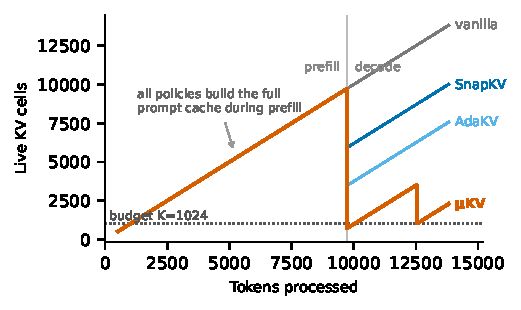
\includegraphics[width=\columnwidth]{fig_cache_trajectory.pdf}
\caption{Live KV cells through prefill and decode on Llama-3.2-1B. Only \muKV\ compacts to its budget and stays bounded.}
\label{fig:cache-trajectory}
\end{figure}

\paragraph{Sustained decode on the CPU.} Table~\ref{tab:cpu} runs a 9.7K-token prompt followed by 4096 generated tokens. Every policy builds the full prompt cache during prefill (Figure~\ref{fig:cache-trajectory}). \muKV\ then compacts to 721 cells, and its re-eviction keeps the cache bounded near 2K. SnapKV can only drop to 5.9K, and vanilla grows without bound. On Llama-3.2-1B the bounded cache buys 24.2 against 5.0\,tok/s, 2.6 times less wall time and 62\% less energy. Its DDR peak is the coolest, 5\C\ below vanilla, at the same vendor-clamped 1.6\,GHz. SnapKV, Ada-KV, H2O and TOVA keep 3.5K to 6.1K cells live at a nominal 1024. That is a 1.6 to 2.8 times reduction, against the 5 to 10 times their papers report. At their own published budgets the gap widens. On 110 LongBench prompts on the phone CPU, SnapKV at 2048 per head keeps 94\% of the cache and H2O at 20\% of the prompt keeps 92\%. TOVA and Ada-KV at 2048 keep 77\% and 71\%. \muKV\ keeps 14\%. They pay the FA-off capture as well. They run at 5.8 to 6.8\,tok/s and 818 to 1094\,mWh, at or above vanilla's energy. StreamingLLM is the control: it compacts to 777 cells, fewer than \muKV, yet runs at 6.6\,tok/s because it stays on the FA-off path in this engine. Retention does not predict speed; the kernel path does. Quality is unchanged. Teacher-forced perplexity on a WikiText slice verified disjoint from the prompt gives 8.198 against 8.023 (vanilla against \muKV) on Llama-3.2-1B. It gives 3.983 against 3.938 on Phi-3-mini and 6.717 against 6.736 on Bonsai-8B. \muKV\ had evicted 92\% of the prompt cache. Weight compression shrinks the static term of per-token traffic; eviction shrinks the growing one. On 1-bit Bonsai-8B (lower block) \muKV\ gives 4.5 times the throughput, 60\% less energy and a DDR peak 9.7\C\ cooler, with no change to its parameters. The lower two blocks run the same text on Phi-3-mini and gemma-2-2b with every baseline at its published budget. There \muKV\ decodes 4.5 and 2.4 times faster than the full cache with 55\% and 40\% less energy, while the baselines keep 85 to 100\% of the cache.

\begin{table}[tb]
\caption{Adreno 840, 12K-token prompt plus 4096 generated tokens, f16 KV for every policy, cold start, median of $n$ runs. Phi-3 rows come from the current build with the driver gate.}
\label{tab:gpu}
\centering\footnotesize
\setlength{\tabcolsep}{3.5pt}
\begin{tabular}{l r r r r r}
\toprule
\textbf{Policy} & \textbf{$n$} & \textbf{Prefill (s)} & \textbf{tok/s} & \textbf{dec\,$\times$} & \textbf{Cells} \\
\midrule
\multicolumn{6}{l}{\emph{Llama-3.2-1B, ctx 16384}} \\
vanilla (full cache) & 3 & 131 & 24.18 & 1.00 & 9741 \\
\textbf{\muKV}       & 3 & 138 & \good{29.77} & \good{1.23} & 723 \\
\muKV, no compaction & 3 & 132 & 25.61 & 1.06 & 723 \\
SnapKV               & 1 & 229 & 4.76 & 0.20 & 6592 \\
Ada-KV               & 1 & 276 & 2.86 & 0.12 & 3519 \\
TOVA                 & 1 & 176 & 4.34 & 0.18 & 4125 \\
H2O                  & 1 & 279 & 3.58 & 0.15 & 6110 \\
StreamingLLM         & 1 & 176 & 5.55 & 0.23 & 777 \\
\midrule
\multicolumn{6}{l}{\emph{Phi-3-mini, ctx 16384}} \\
vanilla (full cache)     & 1 & 471 & 5.05 & 1.00 & 11157 \\
\textbf{\muKV}, in place & 1 & 586 & \good{13.36} & \good{2.64} & 878 \\
StreamingLLM, own budget & 1 & 445 & 10.60 & 2.10 & 2000 \\
Ada-KV, gate promoted    & 1 & 572 & 9.13 & 1.81 & 4326 \\
SnapKV, gate promoted    & 1 & 532 & 5.80 & 1.15 & 10862 \\
H2O, TOVA & \multicolumn{5}{c}{\emph{refused by the gate; their CPU rows stand}} \\
\bottomrule
\end{tabular}
\end{table}

\paragraph{Mobile GPU.} Table~\ref{tab:gpu} runs the same workload on the Adreno 840. The CPU path's state-swap and state-API defrag are not viable here: the swap serializes hundreds of megabytes through host memory, and the Vulkan backend stores FA-off and FA-on caches in different layouts. In-graph scoring removes both needs. Prefill is vanilla-class by construction. \muKV\ decodes at 1.23 times the full cache at 7.4\% of the cells; without compaction the cache stays physically sparse and the gain falls to 1.06. On Llama-3.2-1B every per-head evictor runs at 0.12 to 0.23 times the full cache with 3.5K to 6.6K cells live. On Phi-3-mini the round trip is killed at 16K, while in-place compaction runs there and reaches 2.64 times the full cache on 7.9\% of the cells. Phi-3 also needs a driver gate: the FlashAttention-off capture is numerically broken at head dimension 96, and uncorrected runs decode at full speed while emitting 18 to 44\% corrupted tokens. The gate promotes SnapKV and Ada-KV to the in-graph side node and refuses H2O and TOVA. The two promoted evictors then reach 1.15 and 1.81 times the full cache while holding 97\% and 39\% of it. Quantized KV is numerically invalid on this driver, so every GPU row is f16.

\begin{table}[tb]
\caption{Quality. Needle retrieval on the phone: hits out of 14 depths per model. LongBench F1 on the RTX 4500 Ada: mean over five tasks, and cells kept as a share of the prompt.}
\label{tab:quality}
\centering\scriptsize
\setlength{\tabcolsep}{2.4pt}
\begin{tabular}{l cccc  rrrr}
\toprule
 & \multicolumn{4}{c}{\textbf{Needle hits / 14}} & \multicolumn{4}{c}{\textbf{LongBench F1 (cells kept, \%)}} \\
\cmidrule(lr){2-5}\cmidrule(lr){6-9}
\textbf{Policy} & Phi-3 & Llama & Gemma & Bonsai & Llama & Gemma & Phi-3 & Bonsai \\
\midrule
vanilla & 14 & 13 & 11 & 14 & 42.0 (100) & 50.1 (100) & 54.4 (100) & 48.6 (100) \\
\textbf{\muKV} & \good{14} & \good{13} & \good{11} & \good{14} & \good{42.1 (13)} & 47.3 (13) & \good{54.4 (12)} & 45.0 (13) \\
SnapKV & 14 & 12 & 11 & 14 & 42.7 (82) & 49.7 (94) & 53.6 (83) & 50.0 (96) \\
Ada-KV & 14 & 12 & 11 & 14 & 42.7 (47) & 49.3 (66) & 53.4 (51) & 49.0 (68) \\
TOVA & 14 & 12 & 11 & 14 & 42.8 (54) & 49.6 (67) & 57.5 (55) & 48.7 (73) \\
H2O & 14 & 8 & 10 & 13 & 41.8 (83) & 48.2 (92) & 53.9 (91) & 47.5 (91) \\
StreamingLLM & \bad{3} & \bad{3} & \bad{2} & \bad{3} & 37.6 (23) & 45.8 (31) & 48.2 (21) & 41.2 (25) \\
\bottomrule
\end{tabular}
\end{table}

\begin{figure*}[tp]
\centering

\includegraphics[width=0.96\textwidth]{fig_loop_proof.pdf}
\caption{The two loops provoked on the phone: the lever and plan of thirteen cooled requests (top), and their metered time and energy against budget (bottom). Dark bars are misses.}
\label{fig:loop-proof}
\end{figure*}

\paragraph{Retrieval and long-context quality.} A fact is buried at one of seven depths in 4K or 8K tokens of filler. The 392 cells cover seven policies, four models, seven depths and two contexts (Table~\ref{tab:quality}, left). \muKV\ matches the full cache on every model. It attends to about 1024 cells against 3000 to 3700 for the score-reading evictors and decodes at 17.6 against 8.8\,tok/s over all cells. It is the lowest-energy policy at 307 against vanilla's 309\,mWh, a tie because this 64-token workload is prefill-dominated. StreamingLLM fails retrieval everywhere; its window evicts exactly the middle of the context. Where every policy misses a depth, the full cache misses it too. LongBench (Table~\ref{tab:quality}, right) scores 50 samples per task, with StreamingLLM at its own budget of 2004 cells. \muKV\ keeps 12 to 13\% of the prompt cache. It stays within 0.1 F1 of the full cache on Llama-3.2-1B and Phi-3-mini, and within 2.8 and 3.7 on gemma-2-2b and Bonsai-8B. The per-head evictors score within a point of the full cache at 47 to 96\% of the cache. They are close to the full cache because they nearly are the full cache. The same comparison runs on the device. On the phone CPU, on 103 prompts with each policy at its own published budget, \muKV\ scores 37.0 against the full cache's 36.9 while holding 14\% of the cache. SnapKV, Ada-KV and TOVA gain 0.6 to 1.1 F1 while holding 71 to 94\%.

\begin{figure}[tb]
\centering
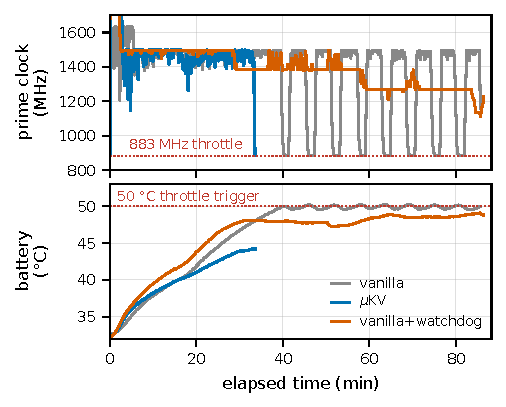
\includegraphics[width=\columnwidth]{fig_bonsai_thermal_2p.pdf}
\caption{Bonsai-8B on the CPU from a cold start: prime clock and battery for the full cache, \muKV, and the full cache with the watchdog (ablation).}
\label{fig:bonsai-thermal}
\end{figure}

\begin{figure}[tb]
\centering

\includegraphics[width=\columnwidth]{fig_discharge_timeline_col.pdf}
\caption{The scheduler through a real discharge: energy and time per request against the battery level it read, with tier bands, the plan chosen and the answer cap. Hatched: cable in.}
\label{fig:discharge}
\end{figure}

\paragraph{Sustained heat and the watchdog.} Figure~\ref{fig:bonsai-thermal} shows the workload that reaches the cliff. The full cache on Bonsai-8B runs 85.6 minutes and drives the battery to 50.2\C. At 50\C\ the vendor deep-throttles both clusters, the prime cores to 883\,MHz, in a sawtooth of 17 dips that spends 923\,s at 883\,MHz in total. \muKV\ finishes in 33.2 minutes at a 44.2\C\ battery peak, before the trigger. Given the watchdog as an ablation, the full cache's battery rise flattens from 0.48 to 0.05\C/min and settles at 49.1\C. The prime cores never reach 883\,MHz. This decode is bandwidth-bound, so the throttle costs no speed (1.0\,tok/s either way): the watchdog buys sustainability, and \muKV\ buys speed. On the GPU, three cooled cells per arm of the 4096-token request give 1289 against 1390\,J and a DDR peak of 75 against 90\C\ for 1\% more time. We also tied the cache budget itself to DDR temperature, a four-tier ladder over $K\in\{256,\dots,1024\}$. The result is negative. Halving $K$ under co-load left peak DDR unchanged, and on a cool phone a smaller cache runs hotter at peak, because the saved bandwidth converts to speed and power. Cache size controls throughput, time and energy; the clock caps heat.

\begin{table}[tb]
\caption{The plan at each battery tier and its cost on the cable (cooled cells) and on the battery (the real discharge). Llama-3.2-1B, 9737-token prompt, GPU.}
\label{tab:energy-aware}
\centering\footnotesize
\setlength{\tabcolsep}{3pt}
\begin{tabular}{l l r r r r}
\toprule
\textbf{Battery} & \textbf{GPU plan} & \textbf{Cap} & \textbf{Cable J} & \textbf{Batt. J} & \textbf{Batt. s} \\
\midrule
mains or above 50\% & 1200, decode 902 & 4096 & 1336 & 885 & 280 \\
21 to 50\%          & 1200, decode 726 & 1024 & 577  & 748 & 210 \\
20\% or below       & 902              & 512  & 500  & 506 & 177 \\
GPU unavailable     & CPU, $K{=}1024$  & tier & 822  & \no & \no \\
\bottomrule
\end{tabular}
\end{table}



\paragraph{Energy-aware scheduling.} Every number here is from the GPU with Llama-3.2-1B and a 9737-token prompt, cooled per cell. The GPU clock cap trades prefill energy for time. From 1200 to 902\,MHz a 4096-token request falls from 1428 to 1154\,J and rises from 221 to 263\,s. The next step to 726\,MHz buys 3\% more energy for 21\% more time, so it is never taken. Decode barely feels the cap, so the split plan, prefill at 1200 and decode at 902, saves 6\% of the request for 1.5\% of time. The CPU clock is not an energy lever: energy per token is flat within 7\% from 883 to 1632\,MHz. Below $K{=}1024$ the cache saves 3 to 4\% while the worst task loses 37 to 42\% of its score. Output length is linear at 0.17 to 0.21\,J per token, which makes the answer cap the largest lever when the length is open. Thirteen cooled requests with real disturbances then exercised the loops (Figure~\ref{fig:loop-proof}). Four idle cores spinning through a mid-tier request pushed its energy 30\% over budget; the energy loop took the lever down twice, and two clean requests decayed it back. An external 726\,MHz cap 12\,s into three low-tier requests, which is what the vendor limiter does, put them 10 to 12\% over their time budget. The performance loop took the lever up to its clamp. The energy loop returned it once the cap was gone.

A loop resident on the phone then ran 123 requests through the scheduler from 91 to 11\%, with charging disabled and no forced state (Figure~\ref{fig:discharge}, Table~\ref{tab:energy-aware}). The scheduler switched on the first request past each threshold. On the battery the tiers cost 885, 748 and 506\,J per request in 280, 210 and 177\,s: 15\% and 43\% less energy than the healthy tier, with time falling 25\% and 37\%. On the battery the phone is a different machine from the phone on the cable. The same healthy request costs 885\,J instead of 1274, because the OEM runs the GPU cooler when unplugged and caps prefill at 726\,MHz within a minute. There the answer cap and the prefill cap carry the saving. A table seeded from cable cells over-predicted battery requests by 36\%; the clipped learning brought it within 2\% in three requests. The mean prediction error over the run was 8.9\% on the battery against 3.7\% on the cable. PowerBench~\cite{cai2026powerbench} and the FUSE study of governors under LLM inference~\cite{zhang2025fusellm} agree with our per-token costs and with the finding that a profiled static setting matches learned governors.

\paragraph{Scope.} All measurements are on one OnePlus 15. The ladder thresholds are device-specific; the calibration protocol generalizes. Energy is total-device energy from the rail and the coulomb counter, so absolute joules hold within about 10\% while orderings hold. Eviction still costs verbatim recall of the spans it drops, even though prediction and retrieval are preserved. The 1-bit kernels return non-finite logits on Adreno, so Bonsai's phone results are CPU results.

\section{Related Work}
\label{sec:related}

Per-head budget allocation is Ada-KV's idea~\cite{feng2025adakv}; we credit it and do not reprove its bound. CriticalKV~\cite{feng2025criticalkv}, DefensiveKV~\cite{feng2025defensivekv} and AhaKV~\cite{gu2025ahakv} refine the score. R-KV~\cite{cai2025rkv} and DynamicKV~\cite{zhou2024dynamickv} argue for task-aware budgets, as our demand-based sizing does. KIVI~\cite{liu2024kivi} and KVzip~\cite{kim2025kvzip} are orthogonal. None reports a temperature, a watt or a resident set on a phone. Among mobile systems, PowerInfer-2~\cite{song2024powerinfer2} and LLM in a Flash~\cite{alizadeh2023llm} optimize weight access. KVSwap swaps the cache to disk on a Jetson, and DynaKV offloads to UFS on the CPU. PerCache~\cite{liu2025percache} shortcuts whole passes at the application level and composes with \muKV. MLC-LLM~\cite{mlcllm}, ExecuTorch and the vendor SDKs use the unmodified cache. Verified from their evaluation sections: the policies that evict run on servers or Jetson boards. The systems that run on phones keep every token. The studies that use a phone GPU apply no cache management. \muKV\ occupies the empty cell. On control, zTT~\cite{kim2021ztt} and FUSE~\cite{liu2022fuse} act on frequency alone. We know of no prior system that reads attention-internal state and battery and thermal sensors in one decode loop on a phone.

\section{Conclusion}
\label{sec:conclusion}

\muKV\ makes attention-driven KV eviction work on a phone by respecting the engine. Scores come from inside the FlashAttention graph. One keep set is what the shared cell array can free. Compaction never needs a second context. A reduce-only clock watchdog keeps the vendor throttle unreachable, and a per-request scheduler with one lever and two loops spends the battery according to its level. On a OnePlus 15 the result is 4.8 times the full cache's decode throughput on the CPU and 1.23 times on the GPU, at 7\% of the cells and 62\% less energy. Retrieval matches the full cache and LongBench nearly does. A real discharge's lower tiers cost 15\% and 43\% less per request. The cache is the phone's efficiency actuator and the clock its temperature actuator. Every per-head budget that looks good on a server is a full cache in disguise on the device.

\begin{thebibliography}{99}
\small
\bibitem{zhang2023h2o} Z. Zhang et al. ``H2O: Heavy-Hitter Oracle for Efficient Generative Inference of LLMs.'' NeurIPS, 2023.
\bibitem{xiao2024streamingllm} G. Xiao et al. ``Efficient Streaming Language Models with Attention Sinks.'' ICLR, 2024.
\bibitem{oren2024tova} M. Oren et al. ``Transformers are Multi-State RNNs.'' arXiv:2401.06104, 2024.
\bibitem{li2024snapkv} Y. Li et al. ``SnapKV: LLM Knows What You're Looking For Before Generation.'' NeurIPS, 2024.
\bibitem{liu2024kivi} Z. Liu et al. ``KIVI: Tuning-Free Asymmetric 2bit Quantization for KV Cache.'' arXiv:2402.02750, 2024.
\bibitem{feng2025adakv} Y. Feng et al. ``Ada-KV: Optimizing KV Cache Eviction by Adaptive Budget Allocation.'' NeurIPS, 2025.
\bibitem{feng2025criticalkv} Y. Feng et al. ``CriticalKV: A Perturbation Perspective on KV Cache Eviction.'' ICML, 2026.
\bibitem{feng2025defensivekv} Y. Feng et al. ``DefensiveKV: Worst-Case Risk Control for KV Cache Eviction.'' ICLR, 2026.
\bibitem{gu2025ahakv} Y. Gu et al. ``AhaKV: Adaptive Holistic Attention-Driven KV Cache Eviction.'' arXiv:2506.03762, 2025.
\bibitem{dao2022flashattention} T. Dao et al. ``FlashAttention: Fast and Memory-Efficient Exact Attention.'' NeurIPS, 2022.
\bibitem{dao2023flashattention2} T. Dao. ``FlashAttention-2: Faster Attention with Better Parallelism.'' arXiv:2307.08691, 2023.
\bibitem{song2024powerinfer2} Y. Song et al. ``PowerInfer-2: Fast LLM Inference on a Smartphone.'' arXiv:2406.06282, 2024.
\bibitem{alizadeh2023llm} K. Alizadeh et al. ``LLM in a Flash: Efficient Inference with Limited Memory.'' arXiv:2312.11514, 2023.
\bibitem{llamacpp} G. Gerganov. ``llama.cpp.'' \url{https://github.com/ggerganov/llama.cpp}.
\bibitem{kim2025kvzip} J.-H. Kim et al. ``KVzip: Query-Agnostic KV Cache Compression with Context Reconstruction.'' NeurIPS, 2025.
\bibitem{liu2025percache} K. Liu et al. ``PerCache: Predictive Hierarchical Cache for RAG Applications on Mobile Devices.'' arXiv:2601.11553, 2025.
\bibitem{mlcllm} MLC Team. ``MLC-LLM: Universal LLM Deployment.'' \url{https://github.com/mlc-ai/mlc-llm}.
\bibitem{kim2021ztt} S. Kim et al. ``zTT: Learning-Based DVFS with Zero Thermal Throttling for Mobile Devices.'' MobiSys, 2021.
\bibitem{liu2022fuse} S. Liu et al. ``FUSE: Fine-Grained Power Management for Mobile Devices.'' SenSys, 2022.
\bibitem{cai2025rkv} X. Cai et al. ``R-KV: Redundancy-aware KV Cache Compression for Reasoning Models.'' arXiv:2505.24133, 2025.
\bibitem{zhou2024dynamickv} X. Zhou et al. ``DynamicKV: Task-Aware Adaptive KV Cache Compression for Long Context LLMs.'' arXiv:2412.14838, 2024.
\bibitem{prismml2026bonsai} PrismML. ``Bonsai: Commercially Viable 1-bit LLMs.'' 2026. \url{https://prismml.com/news/bonsai-8b}.
\bibitem{hoffmann2015jouleguard} H. Hoffmann. ``JouleGuard: Energy Guarantees for Approximate Applications.'' SOSP, 2015.
\bibitem{kim2015racepace} D. H. K. Kim, C. Imes, and H. Hoffmann. ``Racing and Pacing to Idle: Theoretical and Empirical Analysis of Energy Optimization Heuristics.'' CPSNA, 2015.
\bibitem{zou2026enerinfer} B. Zou et al. ``EnerInfer: Energy-Aware On-Device LLM Inference.'' arXiv:2606.23001, 2026.
\bibitem{cai2026powerbench} G. Cai et al. ``Is Your NPU Ready for LLMs? A Power Benchmark of On-Device Inference.'' arXiv:2607.05475, 2026.
\bibitem{zhang2025fusellm} Z. Zhang et al. ``Dissecting the Impact of Mobile DVFS Governors on LLM Inference Performance and Energy Efficiency.'' arXiv:2507.02135, 2025.
\end{thebibliography}

\end{document}
